\documentclass[article]{jss}
\usepackage[utf8]{inputenc}

\author{
Matthieu Stigler\\UC Davis \And Bastiaan Quast\\The Graduate Institute, Geneva
}
\title{\pkg{rddtools}: tools for Regression Discontinuity Design in R}
\Keywords{RDD, Regression, Discontinuity, Design, \proglang{R}}

\Abstract{
The rddtools package implements functions for handling Regression
Discontinuity Design in R.
}

\Plainauthor{Matthieu Stigler, Bastiaan Quast}
\Plaintitle{rddtools: tools for Regression Discontinuity Design in R}
\Shorttitle{\pkg{rddtools}}
\Plainkeywords{RDD, Regression, Discontinuity, Design R}

%% publication information
%% \Volume{50}
%% \Issue{9}
%% \Month{June}
%% \Year{2012}
%% \Submitdate{2012-06-04}
%% \Acceptdate{2012-06-04}

\Address{
    Matthieu Stigler\\
  UC Davis\\
  California\\
  E-mail: \href{mailto:matthieu.stigler@gmail.com}{\nolinkurl{matthieu.stigler@gmail.com}}\\
  URL: \url{https://matthieustigler.github.io/}
      Bastiaan Quast\\
  The Graduate Institute, Geneva\\
  Maison de la paix Geneva, Switzerland\\
  E-mail: \href{mailto:bquast@gmail.com}{\nolinkurl{bquast@gmail.com}}\\
  URL: \url{http://qua.st/}
  }

\usepackage{amsmath}

\begin{document}

\section{Introduction}\label{introduction}

The \texttt{rddtools} package address

\section{Design}\label{design}

A unified framework is implemented through the \texttt{rdd\_data} class
which inherits from the \texttt{R} \texttt{base} \texttt{data.frame}
class. This functionality is made accessible throug hthe associated
\texttt{rdd\_data()} functions and methods.

The package is designed to leveredge of existing implementations of
\textbf{Regression Discontinuity Design} in \texttt{R}, such as the
\texttt{rdd} package.

It implements several variants of RDD previously not implemented.

\begin{itemize}
\itemsep1pt\parskip0pt\parsep0pt
\item
  Simple visualisation of the data using binned-plot: \texttt{plot()}
\item
  Bandwidth selection:

  \begin{itemize}
  \itemsep1pt\parskip0pt\parsep0pt
  \item
    MSE-RDD bandwidth procedure of (G. Imbens and Kalyanaraman 2012):
    \texttt{rdd\_bw\_ik()}
  \item
    MSE global bandwidth procedure of (Ruppert, Sheather, and Wand
    1995): \texttt{rdd\_bw\_rsw()}
  \end{itemize}
\item
  Estimation:

  \begin{itemize}
  \itemsep1pt\parskip0pt\parsep0pt
  \item
    RDD parametric estimation: \texttt{rdd\_reg\_lm()} This includes
    specifying the polynomial order, including covariates with various
    specifications as advocated in (G. W. Imbens and Lemieux 2008).
  \item
    RDD local non-parametric estimation: \texttt{rdd\_reg\_np()}. Can
    also include covariates, and allows different types of inference
    (fully non-parametric, or parametric approximation).
  \item
    RDD generalised estimation: allows to use custom estimating
    functions to get the RDD coefficient. Could allow for example a
    probit RDD, or quantile regression.
  \end{itemize}
\item
  Post-Estimation tools:

  \begin{itemize}
  \itemsep1pt\parskip0pt\parsep0pt
  \item
    Various tools, to obtain predictions at given covariate values (
    \texttt{rdd\_pred()} ), or to convert to other classes, to lm (
    \texttt{as.lm()} ), or to the package \texttt{np} (
    \texttt{as.npreg()} ).
  \item
    Function to do inference with clustered data: \texttt{clusterInf()}
    either using a cluster covariance matrix ( \textbf{vcovCluster()} )
    or by a degrees of freedom correction (as in (Cameron, Gelbach, and
    Miller 2008)).
  \end{itemize}
\item
  Regression sensitivity analysis:

  \begin{itemize}
  \itemsep1pt\parskip0pt\parsep0pt
  \item
    Plot the sensitivity of the coefficient with respect to the
    bandwith: \texttt{plotSensi()}
  \item
    \textbf{Placebo plot} using different cutpoints:
    \texttt{plotPlacebo()}
  \end{itemize}
\item
  Design sensitivity analysis:

  \begin{itemize}
  \itemsep1pt\parskip0pt\parsep0pt
  \item
    McCrary test of manipulation of the forcing variable: wrapper
    \texttt{dens\_test()} to the function \texttt{DCdensity()} from
    package \texttt{rdd}.
  \item
    Test of equal means of covariates: \texttt{covarTest\_mean()}
  \item
    Test of equal density of covariates: \texttt{covarTest\_dens()}
  \end{itemize}
\item
  Datasets

  \begin{itemize}
  \itemsep1pt\parskip0pt\parsep0pt
  \item
    Contains the data set of Arcand (2015): \texttt{indh}
  \item
    Contains the seminal dataset of Lee (2008): \texttt{house}
  \item
    Contains functions to replicate the Monte-Carlo simulations of
    {[}Imbens and Kalyanaraman 2012{]}: \texttt{gen\_mc\_ik()}
  \end{itemize}
\end{itemize}

\section{Application}\label{application}

we use the data from the Initiative Nationale du Development Humaine
(INDH) a development project in Morocco. The data is included with the
\texttt{rddtools} package under the name \texttt{indh}.

\begin{CodeChunk}
\begin{CodeInput}
data("indh")
\end{CodeInput}
\end{CodeChunk}

Now that we have loading the data we can briefly inspect the structure
of the data.

\begin{CodeChunk}
\begin{CodeInput}
summary(indh)
\end{CodeInput}
\begin{CodeOutput}
   choice_pg         commune         poverty     
 Min.   :0.0000   Min.   :28.09   Min.   :28.09  
 1st Qu.:0.0000   1st Qu.:29.01   1st Qu.:29.01  
 Median :1.0000   Median :29.95   Median :29.95  
 Mean   :0.6722   Mean   :29.73   Mean   :29.73  
 3rd Qu.:1.0000   3rd Qu.:30.34   3rd Qu.:30.34  
 Max.   :1.0000   Max.   :30.97   Max.   :30.97  
\end{CodeOutput}
\end{CodeChunk}

The \texttt{indh} object is a \texttt{data.frame} containing 729
observations (representing individuals) of three variables:

\begin{itemize}
\itemsep1pt\parskip0pt\parsep0pt
\item
  \texttt{choice\_pg}
\item
  \texttt{commune}
\item
  \texttt{poverty}
\end{itemize}

The variable of interest is \texttt{choice\_pg}, which represent the
decision to contibute to a public good or not. The observations are
individuals choosing to contribute or not, these individuals are
clustered by the variable \texttt{commune} which is the municiple
structure at which funding was distributed as part of the INDH project.
The forcing variable is \texttt{poverty} which represents the number of
households in a commune living below the poverty threshold. As part of
the INDH, commune with a proportion of household below the poverty
threshhold greater than 30\% were allowed to distribute the funding
using a \textbf{Community Driven Development} scheme. The cutoff point
for our analysis is therefore \texttt{30}.

We can now transform the \texttt{data.frame} to a special
\texttt{rdd\_data} \texttt{data.frame} using the \texttt{rdd\_data()}
function.

\begin{CodeChunk}
\begin{CodeInput}
rdd_dat_indh <- rdd_data(y=choice_pg,
                         x=poverty,
                         data=indh,
                         cutpoint=30 )
\end{CodeInput}
\end{CodeChunk}

The structure is similar but contains some additional information.

\begin{CodeChunk}
\begin{CodeInput}
str(rdd_dat_indh)
\end{CodeInput}
\begin{CodeOutput}
Classes 'rdd_data' and 'data.frame':    729 obs. of  2 variables:
 $ x: num  30.1 30.1 30.1 30.1 30.1 ...
 $ y: int  0 1 1 1 1 1 0 1 0 0 ...
 - attr(*, "hasCovar")= logi FALSE
 - attr(*, "labels")= list()
 - attr(*, "cutpoint")= num 30
 - attr(*, "type")= chr "Sharp"
\end{CodeOutput}
\end{CodeChunk}

In order to best understand our data, we start with an exploratory data
analysis using tables\ldots{}

\begin{CodeChunk}
\begin{CodeInput}
summary(rdd_dat_indh)
\end{CodeInput}
\begin{CodeOutput}
### rdd_data object ###

Cutpoint: 30 
Sample size: 
    -Full : 729 
    -Left : 371 
    -Right: 358
Covariates: no 
\end{CodeOutput}
\end{CodeChunk}

\ldots{}and plots.

\begin{CodeChunk}
\begin{CodeInput}
plot(rdd_dat_indh[1:715,])
\end{CodeInput}


\begin{center}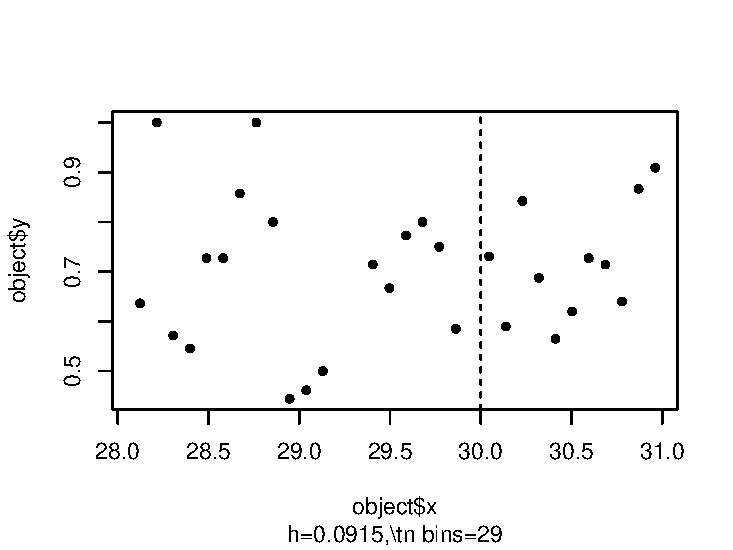
\includegraphics{README_files/figure-latex/unnamed-chunk-7-1} \end{center}

\end{CodeChunk}

We can now continue with a standard Regression Discontinuity Design
(RDD) estimation.

\begin{CodeChunk}
\begin{CodeInput}
(reg_para <- rdd_reg_lm(rdd_dat_indh, order=4))
\end{CodeInput}
\begin{CodeOutput}
### RDD regression: parametric ###
    Polynomial order:  4 
    Slopes:  separate 
    Number of obs: 729 (left: 371, right: 358)

    Coefficient:
  Estimate Std. Error t value Pr(>|t|)
D  0.26428    0.16590   1.593   0.1116
\end{CodeOutput}
\end{CodeChunk}

and visualising this estimation.

\begin{CodeChunk}
\begin{CodeInput}
plot(reg_para)
\end{CodeInput}


\begin{center}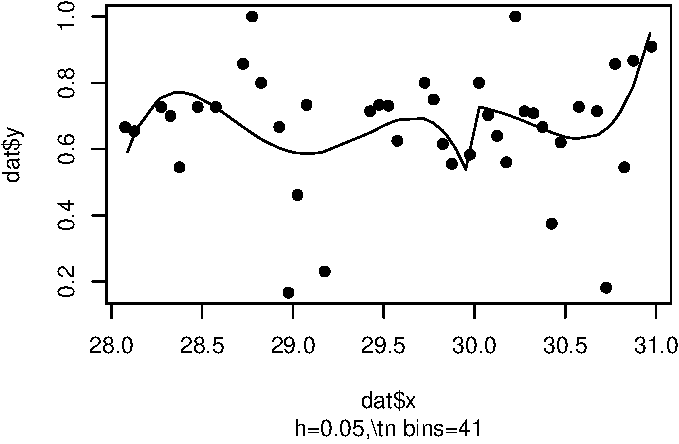
\includegraphics{README_files/figure-latex/unnamed-chunk-9-1} \end{center}

\end{CodeChunk}

In addition to the parametric estimation, we can also perform a
non-parametric estimation.

\begin{CodeChunk}
\begin{CodeInput}
bw_ik <- rdd_bw_ik(rdd_dat_indh)
(reg_nonpara <- rdd_reg_np(rdd_object=rdd_dat_indh, bw=bw_ik))
\end{CodeInput}
\begin{CodeOutput}
### RDD regression: nonparametric local linear###
    Bandwidth:  0.7812904 
    Number of obs: 467 (left: 146, right: 321)

    Coefficient:
  Estimate Std. Error z value Pr(>|z|)  
D 0.178174   0.095319  1.8692  0.06159 .
---
Signif. codes:  0 '***' 0.001 '**' 0.01 '*' 0.05 '.' 0.1 ' ' 1
\end{CodeOutput}
\end{CodeChunk}

and visualising the non-parametric estimation.

\begin{CodeChunk}
\begin{CodeInput}
plot(reg_nonpara)
\end{CodeInput}


\begin{center}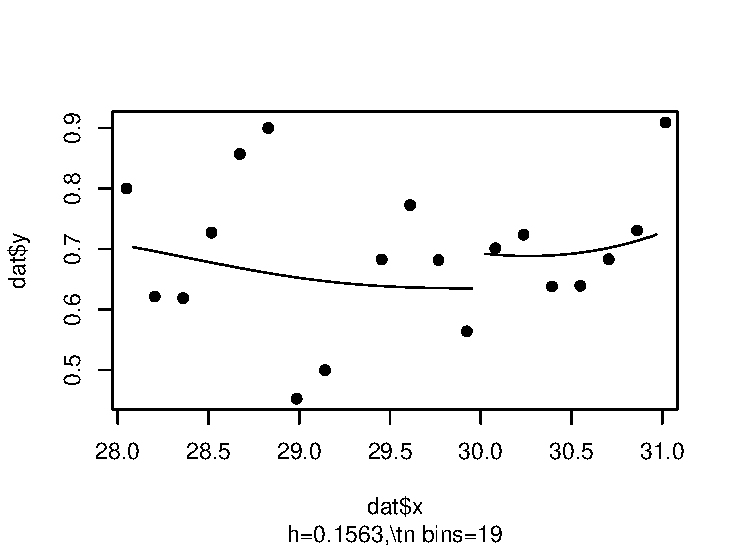
\includegraphics{README_files/figure-latex/unnamed-chunk-11-1} \end{center}

\end{CodeChunk}

Sensitity tests.

\begin{CodeChunk}
\begin{CodeInput}
plotSensi(reg_nonpara, from=0.05, to=1, by=0.1)
\end{CodeInput}


\begin{center}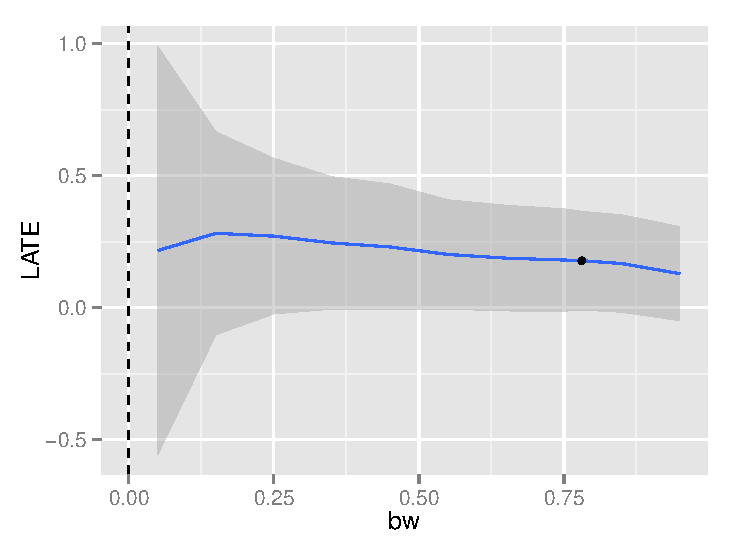
\includegraphics{README_files/figure-latex/unnamed-chunk-12-1} \end{center}

\end{CodeChunk}

\section*{References}\label{references}
\addcontentsline{toc}{section}{References}

Arcand, Rieger, and Nguyen. 2015. ``Development Aid and Social Dyanmics
Data Set.''

Cameron, A Colin, Jonah B Gelbach, and Douglas L Miller. 2008.
``Bootstrap-Based Improvements for Inference with Clustered Errors.''
\emph{The Review of Economics and Statistics} 90 (3). MIT Press:
414--27.

Imbens, Guido W, and Thomas Lemieux. 2008. ``Regression Discontinuity
Designs: A Guide to Practice.'' \emph{Journal of Econometrics} 142 (2).
Elsevier: 615--35.

Imbens, Guido, and Karthik Kalyanaraman. 2012. ``Optimal Bandwidth
Choice for the Regression.''

Lee, David S. 2008. ``Randomized Experiments from Non-Random Selection
in US House Elections.'' \emph{Journal of Econometrics} 142 (2).
Elsevier: 675--97.

Ruppert, David, Simon J Sheather, and Matthew P Wand. 1995. ``An
Effective Bandwidth Selector for Local Least Squares Regression.''
\emph{Journal of the American Statistical Association} 90 (432). Taylor
\& Francis: 1257--70.

\end{document}

